\documentclass{article}
% \usepackage{anyfontsize}
\usepackage{a0size}             % For arbitrary sized font.
\renewcommand{\familydefault}{\sfdefault}
\renewcommand{\tiny}{\fontsize{12}{14}\selectfont}
\renewcommand{\scriptsize}{\fontsize{14.4}{18}\selectfont}
\renewcommand{\footnotesize}{\fontsize{17.28}{22}\selectfont}
\renewcommand{\small}{\fontsize{20.74}{25}\selectfont}
\renewcommand{\normalsize}{\fontsize{24.88}{30}\selectfont}
\renewcommand{\large}{\fontsize{29.86}{37}\selectfont}
\renewcommand{\Large}{\fontsize{35.83}{45}\selectfont}
\renewcommand{\LARGE}{\fontsize{43}{54}\selectfont}
\renewcommand{\huge}{\fontsize{51.6}{64}\selectfont}
\renewcommand{\Huge}{\fontsize{61.92}{77}\selectfont}
\newcommand{\veryHuge}{\fontsize{74.3}{93}\selectfont}
\newcommand{\VeryHuge}{\fontsize{89.16}{212}\selectfont}
\newcommand{\VERYHuge}{\fontsize{107}{134}\selectfont}
\usepackage[
paperwidth=30in,
paperheight=45in,
margin=0.5cm,
head=2.66685in,
foot=1.78685in,
includehead,
includefoot,
%showframe
]{geometry}
\usepackage{fancyhdr}
\title{GPUs for massively parallel mechanistic modeling}
\pagestyle{fancy}
\renewcommand{\headrulewidth}{0pt}
\renewcommand{\footrulewidth}{0pt}
\setlength{\headheight}{2.66685in} % 2.47in + 0.5cm
\fancyhead[L]{%
  \begin{tikzpicture}[%
    background rectangle/.style = {
      fill = fh-blue,
      inner sep = 0pt,
    },
    show background rectangle,
    tight background,
    scale = 1]
    \node (ref) [
    inner sep = 0,
    minimum width = 30in - 1cm,
    minimum height = 2.47in] {};
    \node at (ref.north west) [anchor = north west, name = fh] {%
      \includegraphics[height=2.47in]{fh.png}};
    \node at (ref.south east) [%
    anchor = south east, %
    name = nsf-text,
    text = fh-gold,
    scale = 1.7,
    text width = width("under award number 2231406"),
    align = center] {%
      SGX3 is funded by the \mbox{National Science Foundation} %
      under award number 2231406};
    \path let \p1 = (ref.north), \p2 = (nsf-text.north), \n1 = {\y1 - \y2} in
    node at (nsf-text.north) [anchor = south, name = nsf] {%
      \includegraphics[height=\n1]{nsf.png}};
    \node at (fh.east) [%
    anchor = west,
    text = fh-gold,
    scale = 7,
    text width = width("GPUs for massively parallel")] {%
      GPUs for massively parallel mechanistic modeling%
    };
  \end{tikzpicture}%
}
\fancyhead[C,R]{}
\setlength{\footskip}{1.78685in} % 1.59in + 0.5cm
\fancyfoot[L]{%
  \begin{tikzpicture}[%
    background rectangle/.style = {
      fill = fh-blue,
      inner sep = 0pt,
    },
    show background rectangle,
    tight background,
    scale = 1]
    \pgfdeclarelayer{foreground}
    \pgfsetlayers{background,main,foreground}
    \begin{pgfonlayer}{foreground}
    \node (ref) [
    inner sep = 0,
    minimum width = 30in - 1cm,
    minimum height = 1.59in] {};
    \node (sgx3) at ([xshift=0.5cm]ref.west) [anchor = west] {%
      \includegraphics[height=0.85in]{sgx3.png}};
    \node (ornl) at (sgx3.east) [anchor = west] {%
      \includegraphics[height=1.04in]{ornl.png}};
    \node (omnibond) at (ornl.east) [anchor = west] {%
      \includegraphics[height=0.87in]{omnibond.jpg}};
    \node (tacc) at (omnibond.east) [anchor = west] {%
      \includegraphics[height=0.87in]{tacc.png}};
    \node (qr-code) at (ref.east) [anchor = east, outer sep = 0.25cm] {%
      \includegraphics[height=1.32in]{qr-code.png}};
    \node at (qr-code.west) [anchor = east, text = fh-gold, scale = 3.5] {%
      \textbf{Event Site:} %
      \url{https://hackhpc.github.io/facultyhack-gateways25}
      };
    \end{pgfonlayer}
    \begin{pgfonlayer}{main}
      \node [
      inner sep = 0pt, fit = (sgx3) (ornl) (omnibond) (tacc), fill = white] {};
    \end{pgfonlayer}
  \end{tikzpicture}%
}
\fancyfoot[C]{}

\usepackage{graphicx}
\graphicspath{{img/}}

\usepackage{multicol}
\setlength\columnseprule{0pt}
\setlength{\columnsep}{2.5pc}

\usepackage{tikz}
\usetikzlibrary{
arrows.meta,
backgrounds,
calc,
decorations.markings,
decorations.pathmorphing,
decorations.text,
fit,
mindmap,
tikzmark
}

\usepackage{soul}

\usepackage{amssymb}            % \blacksquare
\usepackage{amsmath}            % \text

\usepackage{tabularx}
\newcolumntype{C}{>{\centering\arraybackslash}X}
\newcolumntype{R}{>{\raggedleft\arraybackslash}X}
% Vertically center within row https://tex.stackexchange.com/a/343329
\renewcommand\tabularxcolumn[1]{m{#1}}
\usepackage{booktabs}
\usepackage{multirow}

\usepackage[
abbreviate=true,
bibencoding=utf8,
minnames=2,
maxbibnames=99,
sorting=none,
style=vancouver,
citestyle=numeric-comp
]{biblatex}
% The vancouver citation style is based on NLM per
% https://tex.stackexchange.com/a/371433
\addbibresource{references.bib}
\renewcommand*{\bibfont}{\footnotesize\selectfont}

\usepackage[
table
]{xcolor}
\definecolor{fh-blue-lighter}{HTML}{EBEFF7}
\definecolor{fh-blue-darker}{HTML}{D4DEED}
\definecolor{fh-blue}{HTML}{005698}
\definecolor{fh-gold}{HTML}{F7E8C9}

\usepackage{tcolorbox}
\newcommand{\sectionbox}[1]{%
  \begin{tcolorbox}[sharp corners,boxrule=0pt,colback=fh-blue,coltext=fh-gold]%
    \section*{#1\vphantom{Yy}}%
  \end{tcolorbox}%
}

\begin{document}

\begin{multicols}{2}

  \sectionbox{Introduction}%
  \noindent
  Graphical Processing Units (GPUs) %
  are integrated into the core architecture %
  of the world's fastest supercomputers %
  that solve the most computationally difficult, %
  mechanistic scientific problems.
  %
  An 8~year, \$1.8~billion effort %
  called the Exascale Computing Project (ECP) %
  involving 2,800 scientists and engineers %
  recently finished modernizing %
  the underlying scientific numerical software %
  to efficiently use this new generation of machines.
  \medskip

  Computing facilities grant access at no cost %
  to these GPU-accelerated%
  \supercite{%
    carter_2014,%
    beckingsale_2019,%
    reinders_2023%
  } machines %
  only to research software engineers and scientists who demonstrate that %
  their computations scale %
  to efficiently use multiple GPUs across many computer servers / nodes.
  %
  Therefore, %
  it is imperative to teach %
  the data parallel software development skills, %
  appropriate domain science methods, and %
  sustainable software practices %
  to enable large scale, GPU-centric computational research.
  \medskip

  Discussion and feedback on this poster from the community %
  can help make this course a success and %
  support similar hands-on learning and teaching endeavors.
  \vspace{\baselineskip}

  %\textcolor{fh-blue}{Target Course Description}
  %\medskip

  \subsection*{\textcolor{fh-blue}{Target Course Description}}

  %\begin{table}
  {
    \rowcolors{1}{fh-blue-lighter}{fh-blue-darker}
    \begin{tabularx}{\linewidth}{>{\bfseries}r X}
      \toprule
      Course Name:
      & GPUs for massively parallel mechanistic modeling\\
      Course Number:
      & TBA\\
      Department:
      & Chemical Engineering\\
      Anticipated Enrollment:
      & 12\\
      Prerequisites:
      & fluent with at least one %
      procedural programming language\\
      Key Content:
      & performance optimization, %
      software development, %
      domain science methods, %
      capstone project\\
      Description:
      & This course trains graduate researchers %
      with ECP-level skills in high performance computing (HPC), %
      using research software engineer (RSE) rigor, %
      and HPC-relevant domain scientific methods.\\
      Project Repo:
      & \small \url{github.com/omsai/facultyhack-gateways25-nanda}\\
      \bottomrule
    \end{tabularx}
    \medskip
  %\end{table}
  }
  %\textcolor{fh-blue}{Goals}
  %\medskip

  \subsection*{\textcolor{fh-blue}{Goals}}
  \begin{itemize}
  \item Setup student \ul{JetStream2 VM} for homework and capstone projects.
  \item Add students to my \ul{ACCESS group} for cluster runs and %
    help them get their own ACCESS allocation.
  \item Teach all C++ classroom exercises inside a \ul{web IDE}. 
  \item Train students to \ul{package their project}.
  \end{itemize}

  \sectionbox{Initial Course Syllabus}%
  \noindent
    \textbf{High-level comparison of topics.}
        %
        Comparison of this course with the %
        2024 Argonne Training Program on Extreme-Scale Computing (ATPESC'24) %
        and the 2025 Lawrence Livermore National Laboratory %
        High Performance Computing Innovation Center (HPC-IC'25) %
        tutorial series.
        \medskip

    \noindent
    \begin{tabularx}{\linewidth}{%
      >{\hsize=.15\hsize\linewidth=\hsize}X %
      >{\hsize=.34\hsize\linewidth=\hsize}R %
      >{\hsize=.16\hsize\linewidth=\hsize}C %
      >{\hsize=.16\hsize\linewidth=\hsize}C %
      >{\hsize=.16\hsize\linewidth=\hsize}C}
      \toprule
      Category
      & Topic
      & This Course & ATPESC'24 & HPC-IC'25\\
      \midrule
      \multirow{3}{\hsize}{Performance optimization}
      & Within node
      & \checkmark & \checkmark & $\times$\\
      & Multi-node
      & \checkmark & \checkmark & \checkmark\\
      & GPU performance portability
      & \checkmark & \checkmark & \checkmark\\
      \midrule
      \multirow{7}{\hsize}{Software development}
      & Unit testing
      & \checkmark & \checkmark & $\times$\\
      & Performance testing
      & \checkmark & \checkmark & \checkmark\\
      & Continuous integration
      & \checkmark & $\times$ & \checkmark\\
      & Checkpointing
      & \checkmark & $\times$ & \checkmark\\
      & Parallel debugging
      & \checkmark & \checkmark & $\times$\\
      & Code peer review
      & \checkmark & $\times$ & $\times$\\
      & Reproducibility
      & \checkmark & \checkmark & \checkmark\\
      \midrule
      \multirow{-1.5}{\hsize}{Domain science methods}
      & \mbox{Gradient-free optimization\ldots{}} \mbox{\ldots{}of model parameters}
      & \checkmark & $\times$ & \checkmark\\
      & Coupling AI, cloud, data sci.
      & \checkmark & $\times$ & \checkmark\\
      \midrule
      Sysadmin
      & Cluster launch
      & \checkmark & $\times$ & \checkmark\\
      \bottomrule
    \end{tabularx}
    \bigskip

  \sectionbox{Modified Course Syllabus}

    \bigskip
    \begin{minipage}[c]{.23\linewidth}
      \textbf{Course topics.}
          %
          The topics covered in this planned course %
          are organized into the categories of the %
          \textcolor{red!80!black}{$\blacksquare$}~capstone project,
          \textcolor{orange!90!black}{$\blacksquare$}~performance optimization, %
          \textcolor{blue!80!black}{$\blacksquare$}~software development, %
          \textcolor{green!50!black}{$\blacksquare$}~domain science methods, and %
          \textcolor{black!60}{$\blacksquare$}~cluster administration.
          %
          Each leaf node more-or-less corresponds to %
          a single classroom session.
    \end{minipage}
    %\hfill
    \begin{minipage}[c]{.77\linewidth}
      \begin{tikzpicture}[
        root concept/.style={
          text width = 120pt,
        },
        level 1 concept/.style={
          text width = 80pt,
          level distance = 180,
        },
        level 2 concept/.append style={
          text width = 70pt,
          level distance = 120,
        },
        every concept/.append style={
          font = \scriptsize,
        },
        mindmap,
        ]
        \path
        node [concept, concept color=black, text=white, name=node-concept]
        {course topics}
        child [grow=90, concept color=red!80!black, text=white] {
          node [concept] {capstone}
          [clockwise from=210]
          child { node [concept] {present} }
          child { node [concept] {write proposal} }
          child { node [concept] {submit code} }
          child { node [concept] {write abstract} }
        }
        child [grow=18, concept color=orange!90!black, text=white] {
          node [concept] {performance optim.}
          [clockwise from=90]
          child { node [concept] {within node} }
          child { node [concept] {multi node} }
          child { node [concept] {GPU accel.} }
          child { node [concept] {tuning} }
        }
        child [grow=306, concept color=blue!80!black, text=white] {
          node [concept] {software dev.}
          [clockwise from=0]
          child { node [concept] {test, CI} }
          child { node [concept] {debug, checkpoint} }
          child { node [concept] {peer review, reproduce} }
        }
        child [grow=234, concept color=green!50!black, text=white] {
          node [concept] {domain methods}
          [counterclockwise from=205]
          child { node [concept] {coupling AI,~cloud, data sci.} }
          child { node [concept] {scientific param. optim.} }
        }
        child [grow=162, concept color=black!60, text=white] {
          node [concept] {cluster admin.}
          [counterclockwise from=125]
          child { node [concept] {launch} }
          child { node [concept] {profile} }
        };
        \draw [%
        very thick,
        {Circle[length=0.5em]-Stealth[harpoon,length=1em]},
        postaction={
          decorate,
          decoration={
            text align={left},
            raise={0.5em},
            text along path,
            text={Start}
          }
        },
        postaction={
          decorate,
          decoration={
            text align={right},
            raise={0.5em},
            text along path,
            text={End}
          }
        }]
        ([shift=(66:15em)]node-concept) arc (66:-275:15em);
      \end{tikzpicture}
    \end{minipage}


  \sectionbox{Mentors Suggestions}%
  \begin{multicols}{2}
    \begin{enumerate}
    \item \ul{Added network communication exercises} %
      using the LAMMPS exercise developed at Temple University.
    \item \ul{Added profiling exercises} %
      from Cornell University %
      and the University of Michigan.
    \item \ul{Chose a checkpointing library} %
      written in C/C++ %
      both to teach in the course %
      and to recommend for student capstone projects.
    \item Trainees will \ul{write C/C++ code using VS Code} %
      with SSH tunnels to JetStream2 virtual machines %
      with a fallback of OpenVSCode Server web interface %
      for classroom instruction.
    \item \ul{Added an AI policy} %
      that requires a bibliography %
      citing AI service names with versions, prompts, and output.
    \item Moved non-capstone homework assignments to %
      \ul{classroom hands-on to avoid over-reliance on AI support} %
      while trainees are still developing expertise.
    \item \ul{Increased accessibility} %
      to less experienced C/C++ programmers %
      by recommending self-guided, open access textbooks %
      from \emph{The Art of HPC: Volume 3}.
    \item \ul{Added objective of numerical correctness} %
      but limited goal to unit tests, performance test, and CI %
      instead of considering formal methods.
    \item The target audience is now \ul{graduate students} %
      with existing projects or pilot projects.
    \item \ul{Consolidated course topics} %
      to allow for more focus on domain science methods %
      in keeping with the course title.
    \end{enumerate}
  \end{multicols}

  \sectionbox{Science Gateways Resources Used}%
  \begin{description}
  \item[JetStream2-GPU:] non-virtual multi-GPU A100 nodes (g3.2xl)
    \begin{itemize}
    \item Shared between small groups of 4 students.
    \item For early project development and exercises.
    \item A100 supports FP64 for capstone projects that need it.
    \item Efficient multi-GPU use is a course objective.
    \item g3.2xl is the multi-GPU A100 with the most availability.
    \end{itemize}
  \item[ACCESS CI:] Bridges-2 GPU HPC Allocation
    \begin{itemize}
    \item For cluster exercises and scaling.
    \item Interactive nodes with backfill scheduling and short walltime %
    for the classroom use.
    \end{itemize}
  \item[GitHub Workflows:] Trainee repositories for assignments and projects
    \begin{itemize}
    \item Projects in private git repositories shared with the instructor.
    \item Assignments will be partially checked using GitHub workflows.
    \item Progress on capstone projects will be monitored from git repositories.
    \end{itemize}
  \end{description}

  \sectionbox{Expansions}%
  \begin{multicols}{2}
    \begin{enumerate}
    \item Accommodate \ul{undergraduate students} %
      with more structure, %
      shorter exercises, %
      and allow them to choose from a set of smaller capstone projects.
    \item For the last ``fun'' topic before final presentations %
      \ul{launch the cluster using Raspberry Pis}, %
      networking hardware, and network storage %
      for a more memorable hands-on lesson.
    \item Develop an \ul{time-saving exercise for model comparison} %
      to demonstrate the usefulness %
      of detailed benchmarking and analysis tools %
      \ul{to rapidly iterating model development}.
    \item Create \ul{interactive trivial exercises in a web page} %
      to encourage trainee progress with %
      a live updating grading rubric %
      and suggestions to correct common errors.
    \item \ul{Compartmentalize topics %
      into the 2-day workshop format} %
      to be taught at the Pittsburgh Supercomputing Center (PSC).
    \end{enumerate}
  \end{multicols}

  \sectionbox{References}
  {
    % Recalculate \columnsep instead of using the large \columnsep
    % from the main document.
    \setlength{\columnsep}{1.5pc}
    \begin{multicols}{2}
      \printbibliography[heading=none]{}
    \end{multicols}
  }

  \sectionbox{Authors}%
  {
    \setlength{\parindent}{5em}

    \textbf{\textcolor{fh-blue}{\tikzmark{pn}Nanda, Pariksheet}}

    Role: Faculty Participant

    University of Pittsburgh

    pan79@pitt.edu
    \vspace{\baselineskip}

    \textbf{\textcolor{fh-blue}{\tikzmark{em}MacCarthy, Elijah}}

    Role: Community Mentor

    Oak Ridge National Laboratory

    maccarthyea@ornl.gov
  }
  \begin{tikzpicture}[%
    remember picture,
    overlay]
    \node at (pic cs:pn) [%
    anchor = north east,
    yshift = \baselineskip] {%
    \includegraphics[%
    keepaspectratio,
    width=10em,
    height=5em,
    clip,
    trim={55 85 50 35}]{%
        pariksheet.png}};

    \node at (pic cs:em) [%
    anchor = north east,
    yshift = \baselineskip] {%
    \includegraphics[%
    keepaspectratio,
    width=10em,
    height=5em,
    clip,
    trim={20 80 60 5}]{%
        elijah.jpg}};
  \end{tikzpicture}

\end{multicols}

\end{document}
